\documentclass[a4paper, 12pt]{report}

%% Preambles
\usepackage{amsmath}

\usepackage{cite}

% The hyperlinks will not show up when you are working in draft mode
\usepackage{color} 
\usepackage{hyperref}
\definecolor{linkcolour}{rgb}{0,0.2,0.6}
\hypersetup{colorlinks,breaklinks,urlcolor=linkcolour, linkcolor=linkcolour}

% tikz package
\usepackage{graphicx}	% \resizebox
\usepackage{amstext, bm}
\usepackage{tikz}
\usetikzlibrary{arrows,decorations.pathmorphing,fit,positioning, shapes}
% see tikz examples: https://tex.stackexchange.com/questions/328733/how-to-draw-recurrent-neural-network

\usepackage{subfigure}

\begin{document}
\chapter{Recurrent Neural Networks}

%%%%%%%%%%%%%%%%%%%%%%%%%%
\section{Introduction}
A \textbf{recurrent neural network (RNN)} \cite{Rumelhart_1986}, e.g. Fig. \ref{fig:RNN}, is a class of artificial neural network for modelling time series.
The structure of the network is similar to that of a standard  \href{https://en.wikipedia.org/wiki/Feedforward_neural_network}{feedforward neural networks}, with the distinction that it allows connections among hidden units associated with a time delay.
Through these connections the model can retain information about the past, enabling it to discover temporal correlations between events that are far away from each other in the data.

While in principle the recurrent network is a simple and powerful model, in practice, it is hard to train properly. 
Among the main reasons why this model is so unwieldy are the \emph{vanish gradient} and \emph{exploding gradient} problems described in \cite{Bengio2002Learning}. 
In this report, we will analyse these issues thoroughly and summarise those relevant solutions.

%Unlike \href{https://en.wikipedia.org/wiki/Feedforward_neural_network}{feedforward neural networks}, RNNs can use their internal state(memory) to process sequences. 
%This makes them applicable to tasks such as unsegmented, connected handwritten recognition or speech recognition.
% a finite impulse recurrent neural network is a directed acyclic graph that can be unrolled and replaced with a strictly feedforward neural network.

\begin{figure}[htp]
  \centering
   \resizebox{0.6 \textwidth}{!}{
  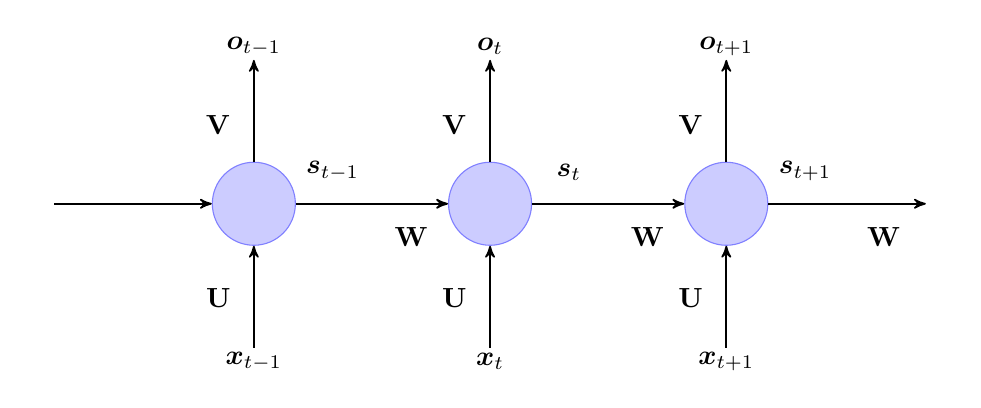
\begin{tikzpicture}
    [
      observed/.style={minimum size=30pt,circle,draw=blue!50,fill=blue!20},
      unobserved/.style={minimum size=30pt,circle,draw},
      hyper/.style={minimum size= 0.1pt,circle},
      hid/.style={minimum size=30pt,circle,draw=blue!50,fill=blue!20},
      post/.style={->,>=stealth',semithick},
      node distance= 1cm and 2cm,
      auto
    ]
    
    \node (nodet) [hid] at (0,0) {};
    \node (nodet_) [hid] at (-3, 0) {};
    \node (nodet+) [hid] at (+3, 0) {};
    \node (xt) [hyper, label=center: $\bm{x}_t$] at (0, -2) {};
    \node (xt_) [hyper, label=center: $\bm{x}_{t-1}$] at (-3, -2) {};
    \node (xt+) [hyper, label=center: $\bm{x}_{t+1}$] at (+3, -2) {};
    \node (ot) [hyper, label=center: $\bm{o}_{t}$] at (0, 2) {};
    \node (ot_) [hyper, label=center: $\bm{o}_{t-1}$] at (-3,2) {};
    \node (ot+) [hyper, label=center: $\bm{o}_{t+1}$] at (3, 2) {}; 
    \node (ht__) [hyper, left =of nodet_] {};
    \node (ht++) [hyper, right =of nodet+] {};
    \node (ht) [hyper, label=above: $\bm{s}_{t}$] at (1, 0) {};
    \node (ht_) [hyper, label=above: $\bm{s}_{t-1}$] at (-2, 0) {};
    \node (ht+) [hyper, label=above: $\bm{s}_{t+1}$] at (4,0) {};
    \node (Vt_) [hyper, label=left: $\mathbf{V}$] at (-3, 1) {};
    \node (Vt) [hyper, label=left: $\mathbf{V}$] at (0, 1) {};
    \node (Vt+) [hyper, label=left: $\mathbf{V}$] at (3, 1) {};
    \node (W_) [hyper, label=below: $\mathbf{W}$] at (-1, 0) {};
    \node (W) [hyper, label=below: $\mathbf{W}$] at (2, 0) {};
    \node (W+) [hyper, label=below: $\mathbf{W}$] at (5, 0) {};
    \node (U_) [hyper, label=left: $\mathbf{U}$] at (-3, -1.2) {};
    \node (U) [hyper, label=left: $\mathbf{U}$] at (0, -1.2) {};
    \node (U) [hyper, label=left: $\mathbf{U}$] at (3, -1.2) {};
    
    
    \path
    (nodet_) edge [post] (nodet)
    (nodet)  edge [post] (nodet+)
    (xt)	edge [post] (nodet)
    (xt_)	edge [post] (nodet_)
    (xt+)	edge [post] (nodet+)
    (nodet)	edge [post] (ot)
    (nodet_) edge [post] (ot_)
    (nodet+) edge [post] (ot+)
    (ht__) 	edge [post] (nodet_)
    (nodet+) edge [post] (ht++)
    ;

  \end{tikzpicture}
  }
  \caption{Schematic of an unrolled recurrent neural network. The recurrent connections in the hidden layer allow information to persist from one input to another.}
  \label{fig:RNN}
\end{figure}

%%%%%%%%%%%%%%%%%%%%%%%%%%
\section{Problem Formulation}
We will make use of the following forward propagation formula\footnote{For any model respecting Eqs. (\ref{Eq::abstraction}, \ref{Eq::activation}), it is widely known as the following two recurrent formulations: $\bm{s}_t = f(\textbf{U} \bm{x}_t + \textbf{W} \bm{s}_{t-1})$ and $\mathrm{net}_t = \textbf{U}\bm{x}_t + \textbf{W} f(\textrm{net}_{t-1})$.} for a recurrent neural network with input $\bm{x}_t$ and state $\bm{s}_t$ at time step $t$: 
\begin{align}
\mathrm{net}_t &= \textbf{U} \bm{x}_t + \textbf{W} \bm{s}_{t-1}  \label{Eq::abstraction} \\
\bm{s}_{t-1} &= f(\mathrm{net}_{t-1}) \label{Eq::activation}
\end{align}
where $\textbf{U}$ and $\textbf{W}$ are the weight matrices connecting the input  $\bm{x}_t$ and the hidden state $\bm{s}_t$ at time step $t$, respectively. 
Also, the neuron output at time step $t$ is represented as $\mathrm{net}_t$.

\subsection{Backpropagation Through Time (BPTT)}
\subsubsection{Element-wise calculus formulation}
Let the $j$th element of the state vector $\bm{s}_t$ to be denoted as $s_{j}^t$, let the $j$th element of the input vector $\bm{x}_t$ be $x_j^{t}$, and similarly the $i$th neuron output is $\mathrm{net}^t_{i}$.
Then the above equation can be written equivalently as
\begin{align}
\mathrm{net}^t_{i} &= u_{i\hat{j}} x^t_{\hat{j}}+ w_{i\hat{j}} s^{t-1}_{\hat{j}} \\
s^{t-1}_j &= f(\mathrm{net}^{t-1}_j)
\end{align}
where the summation $\sum$ is omitted and  by convention it is applied to the hatted indexes.

Let $\delta_{i}^t \equiv \frac{\partial{\mathcal{E}_n}}{\partial{\mathrm{net}_i^t}}$, then the backpropagation through time (BPTT) update formula is derived as the following
\begin{align}
	\delta_i^t &= \frac{\partial{\mathcal{E}_n}}{\partial{\mathrm{net}_{\hat{j}}^{t+1}}} \frac{\partial {\mathrm{net}_{\hat{j}}^{t+1}}}{\partial {\mathrm{net}_i^{t}}} \notag \\
	&= \delta_{\hat{j}}^{t+1} \frac{\partial {\mathrm{net}_{\hat{j}}^{t+1}}}{\partial{s^t_{i}}}  \frac{\partial{s^t_i}} {\partial {\mathrm{net}_i^{t}}} \notag \\
	&= f^{'}(\mathrm{net}^{t}_{i}) ( w_{\hat{j}i} \delta_{\hat{j}}^{t+1}),
\end{align}

or in matrix form as
\begin{align}
\bm{\delta}_t &= \mathrm{diag}(f'(\mathrm{net}^t)) \textbf{W}^\top \bm{\delta}^{t+1} \\
&= (\prod_{l=t}^{T-1} \mathrm{diag}(f'(\mathrm{net}^l)) \textbf{W}^\top) \bm{\delta}_{T}
\end{align}

Now we need to calculate the gradient with respect to each weight entry. Note that
\begin{align}
\frac{\partial {\mathcal{E}_n}}{\partial {w}_{ij}} &= \frac{\partial {\mathcal{E}_n}}{\partial {\mathrm{net}_{i}^{\hat{t}}}} \frac{\partial {\mathrm{net}_{i}^{\hat{t}}}}{\partial {w}_{ij}}  \tag{summation is over $t$} \\
&= \delta_{i}^{\hat{t}} s_{j}^{\hat{t}-1} \label{eq::dwij}
\end{align}
From this equation, we can construct the gradient $\nabla_{\textbf{W}} \mathcal{E}_n$ that are the sum of  the gradients $\nabla_{\textbf{W}_t} \mathcal{E}_n$ at all time step $t$. 

\subsubsection{Matrix calculus formulation}
In this section, we provide a tensor calculus formulation \cite{Kolda2009Tensor} for the BPTT method. 
We summarise some of the tensor notations as follows.

The number of dimensions of a tensor is called as its \emph{order}, it is also known as ways or modes.
Higher-order tensors (order three or higher) are denoted by boldface Euler script letters, e.g., $\mathcal{X}$. 
And the element $(i,j,k)$ of a third-order tensor $\mathcal{X}$ is denoted by $x_{ijk}$. 
Indices typically range from $1$ to their capital version, e.g., $i=1, \ldots, I$. 
The $n$th element in a sequence is denoted by a superscript in parentheses, e.g., $\mathbf{A}^{(n)}$ denotes $n$th matrix in a sequence.

\emph{Fibers} are the higher-order analogue of matrix rows and columns.
A fiber is defined by fixing every index but one. 
A  matrix column is a mode-1 fiber and a matrix row is a mode-2 fiber.
Third-order tensors have column, row, and tube fibers, denoted by $\bm{x}_{:ik}, \bm{x}_{i:k}$ and $\bm{x_{ij:}}$, respectively; see Figure \ref{subfigure::fibers}. 
When extracted from the tensor, fibers are always assumed to be oriented as column vectors. 

\emph{Slices} are two-dimensional sections of a tensor, defined by fixing all but two indices. 
Figure \ref{subfigure::slices} shows the horizontal, lateral, and frontal slides of a third-order tensor $\mathcal{X}$, denoted by $\textbf{X}_{i::}, \textbf{X}_{:j:}$, and $\textbf{X}_{::k}$, respectively.

\newcommand*{\mypicwidth}{14cm}
\begin{figure*}[htp]
\centering
\subfigure[Tensor fibers]{ \label{subfigure::fibers}
	\includegraphics[trim={0cm 0cm 0cm 0cm}, clip=true, width=\mypicwidth]{./figures/tensor_fibers}}
	\hspace{4pt}
\subfigure[Tensor slices]{ \label{subfigure::slices}
	\includegraphics[trim={0cm 0cm 0cm 0cm}, clip=true, width=\mypicwidth]{./figures/tensor_slices}}
\caption{Fibers and slices of a 3rd-order tensor}
\end{figure*}


Now we return to our discussion of BPTT method. 
Let the error signal $\bm{\delta}_t$ at time step $t$ to be defined as  $\frac{\partial {\mathcal{E}_n}}{\partial {\mathrm{net}_t}}$, we then have
\begin{align}
\bm{\delta}_t &=  \frac{\partial {\mathcal{E}_n}}{\partial{\mathrm{net}_{t+1}}}  \frac{\partial{\mathrm{net}_{t+1}}}{\partial{\mathrm{net}_{t}}}  \tag{\href{https://en.wikipedia.org/wiki/Matrix_calculus}{numerator layout}} \\
&= \bm{\delta}_{t+1}  \frac{\partial{\mathrm{net}_{t+1}}}{\partial \bm{s}_t}  \frac{\partial \bm{s}_t}{\partial{\mathrm{net}_{t}}}  \notag \\
&= \bm{\delta}_{t+1} \textbf{W} \mathrm{diag}{(f'(\mathrm{net}_t))} \\
&= \bm{\delta}_T (\prod_{l=t}^{T-1} \textbf{W} \mathrm{diag}(f'(\mathrm{net}_t)))
\end{align}

The update for the weight matrix $\textbf{W}$ is calculated as
\begin{align}
\frac{\partial {\mathcal{E}_n}}{\partial {\textbf{W}}} &=  \frac{\partial {\mathcal{E}_n}}{\partial {\mathrm{net}_{T}}} \frac{\partial {\mathrm{net}_T}}{\partial {\textbf{W}}} \notag \\
&=  \frac{\partial {\mathcal{E}_n}}{\partial {\mathrm{net}_{T}}} \frac{\partial {(\textbf{U} \bm{x}_T + \textbf{W} f(\mathrm{net}_{T-1})})}{\partial {\textbf{W}}} \notag \\
&= \bm{\delta}^{\top}_T \left[ \frac{\partial {\textbf{W}}}{ \partial {\textbf{W}}} \bm{s}_{T-1} + \frac{\partial {\mathrm{net}_T}}{\partial {\mathrm{net}_{T-1}}} \frac {\partial {\mathrm{net}_{T-1}}}{\partial{\textbf{W}}}\right] \notag \\
&=  \bm{\delta}^{\top}_T  \frac{\partial {\textbf{W}}}{ \partial {\textbf{W}}} \bm{s}_{T-1} +  \frac{\partial {\mathcal{E}_n}}{\partial {\mathrm{net}_{T-1}}} \frac {\partial {\mathrm{net}_{T-1}}}{\partial{\textbf{W}}} \notag  \\
&=  \sum_{t=1}^{T} \bm{\delta}^{\top}_t  \frac{\partial {\textbf{W}}}{ \partial {\textbf{W}}} \bm{s}_{t-1}.
\end{align}

Similarly, we have
\begin{align}
\frac{\partial {\mathcal{E}_n}}{\partial {\textbf{U}}} &=  \frac{\partial {\mathcal{E}_n}}{\partial {\mathrm{net}_{T}}} \frac{\partial {\mathrm{net}_T}}{\partial {\textbf{U}}} \notag \\
&=  \frac{\partial {\mathcal{E}_n}}{\partial {\mathrm{net}_{T}}} \frac{\partial {(\textbf{U} \bm{x}_T + \textbf{W} f(\mathrm{net}_{T-1})})}{\partial {\textbf{U}}} \notag \\
&= \bm{\delta}^{\top}_T \left[ \frac{\partial {\textbf{U}}}{ \partial {\textbf{U}}} \bm{x}_{T} + \frac{\partial {\mathrm{net}_T}}{\partial {\mathrm{net}_{T-1}}} \frac {\partial {\mathrm{net}_{T-1}}}{\partial{\textbf{U}}}\right] \notag \\
&=  \bm{\delta}^{\top}_T  \frac{\partial {\textbf{U}}}{ \partial {\textbf{U}}} \bm{x}_{T} +  \frac{\partial {\mathcal{E}_n}}{\partial {\mathrm{net}_{T-1}}} \frac {\partial {\mathrm{net}_{T-1}}}{\partial{\textbf{U}}} \notag  \\
&=  \sum_{t=1}^{T} \bm{\delta}^{\top}_t  \frac{\partial {\textbf{U}}}{ \partial {\textbf{U}}} \bm{x}_{t}.
\end{align}

Note that $\frac{\partial {\textbf{W}}} {\partial {\textbf{W}}}$ is a four way tensor. 
We denote this tensor as $\mathcal{Y}$, then its $(i,j,k,l)$th element is computed as $y_{ijkl} = \frac{\partial {w_{ij}}}{\partial {w_{lk}}}$. 
The generalised formula $\bm{a}^{\top} \mathcal{Y}\bm{b} $ is thus a matrix of $J$ rows and $K$ columns. 
This $jk$th element is calculated as
\begin{align}
a_{\hat{i}} y_{\hat{i}jk\hat{l}} b_{\hat{l}} & = a_{\hat{i}} \frac{\partial {w_{\hat{i}j}}}{\partial {w_{\hat{l}k}}} b_{\hat{l}} \notag \\
& = a_{\hat{i}} (\frac{\partial {w_{\hat{i}j}}}{\partial {w_{\hat{l}k}}} b_{\hat{l}})  = a_{\hat{i}} \frac{\partial {w_{\hat{i}j}}}{\partial {w_{jk}}} b_{j} = a_{k} \frac{\partial {w_{kj}}}{\partial {w_{jk}}} b_{j} \tag{eliminating the zero terms} \\
& = a_{k}  b_{j}
\end{align}
From here, we conclude that  the  equivalent result of Eq. (\ref{eq::dwij})  is obtained.

\subsection{Gradient Vanish and Gradient Exploding}



%%%%%%%%%%%%%%%%%%%%%%%%%%
\bibliographystyle{IEEEtran}
\bibliography{My_Library}

\end{document}